\chapter{The Carlifornia Planet Survey Doppler Code}\label{chap:doppler}

This chapter contains a brief documentation describing the algorithm
and structure of the California Planet Survey (CPS) Doppler code,
which extracts RVs from iodine-calibrated stellar spectra. As of March
2016, no documentation in published or unpublished form existed for
this widely used code, although \cite{butler1996} describes the basics
for the technique of iodine-calibrated precise RV, and some CPS
publications contain description for certain elements of the code
\citep[e.g.,][]{2006ApJ...647..600J, 2009ApJ...696...75H, 2011ApJ...726...73H,
  2011ApJS..197...26J}.

% history of the code
Earliest documentation of code indicates 1991, co-created by Paul
Butler and Geoff Marcy. Heavily modified by John Johnson for CPS. Paul
Butler also has a version for LCPS, which he now maintains and also
serves as the pipeline for PFS and APF. Later maintained by Howard
Issacson at Berkeley. This code has been applied to data taken by
Keck/HIRES, AAT, APF, PFS, Lick/Hamilton, Magellan, HET/HRS (this
thesis), and so on. Our code is from John Johnson, version 2013.


%%%%%%%%%%%%%%%%%%%%%%%%%%%%%%%%%%%%%%%%%%%%%%%%%%%%%%%%%%%%%%%%%%%%%%%%%%%%%%
% basic algorithm, in mathematical form
\section{Basic Formulae, Algorithm, and Components}

First, we describe the basic mathematics and algorithm behind RV
extraction from iodine-calibrated stellar spectra using the CPS
code. The overall algorithm is to forward model the stellar spectra
using synthetic or empirically derived reference spectra, fitting $N$
parameters, one of which is the Doppler shift, $z$.

The reference spectra include\footnote{It can also include a model
  spectrum for a faint secondary star, telluric absorption lines (see
  Chapter~\ref{chap:keck} Section~\ref{keck:sec:telluric}), and so
  on.}: a model spectrum for the iodine absorption lines, $F_{\rm
  I_2}(\lambda)$ and a model spectrum for the star,
$F_{*}(\lambda)$. The goal is to use the model the observed,
extracted, and normalized 1-D spectrum, $F_{\rm obs}(x)$, at any given
pixel position (and spectral order), $x$, using these reference spectra
and model parameters. The broadening effect of the spectrograph is
described by the spectral response function, or the spectral point
spread function, or the instrumental profile (IP), which we will refer
to as the IP throughout this thesis and is denoted as
$\curlyp(x)$. Hence,
\beq
F_{\rm obs}(x) = \left[ F_{\rm I_2}(\lambda(x)) \times
F_{*}'(\lambda(x)) \right] \ast \curlyp(x),
\eeq
where $\lambda(x)$ is the wavelength solution for the 1-D spectrum,
and $F_{*}'$ is the red-shifted stellar spectrum defined by
$F_{*}'(\lambda) = F_{*}(\lambda\cdot(1+z))$. The Doppler shift $z$
contains two components: the stellar RV $v_*$ and the barycentric (BC)
velocity of the Earth $v_{\rm BC}$. The BC component is corrected by
$v_* = v_{\rm measured} + v_{\rm BC} + z \cdot v_{\rm BC}$.

% relative RV measurement to DSST
The stellar reference spectrum is empirically derived from iodine-free
stellar observations taken on an epoch, say, $T_0$. As a result, all
measured RVs for the star using a stellar template from $T_0$
represent relative stellar velocities between epoch $T_0$ and epoch
$T_{\rm obs}$ (i.e., $v_{*,T_{\rm obs}} - v_{*,T_0}$), instead of the
absolutely RVs of the star. The following subsection describes the
origins of the stellar (and also the iodine) reference spectra.



%----------------------------------------------------------------
% Table: RV Forward Modeling Parameters
\renewcommand{\arraystretch}{1.2} % more row spacing for the table
\begin{deluxetable}{ll}
\tabletypesize{\scriptsize}
\tablecaption{Parameters for Forward Modeling \keck\ RV Spectra\label{doppler:tab:rvpar}}
\tablewidth{320pt}
\tablehead{
  \colhead{Parameter} & \colhead{Unit and Meaning}
}
\startdata
$z$ & no unit, the stellar red shift \\
$w_0$ & \AA, wavelength of the first pixel of a spectral chunk \\
$w_d$ & \AA$/$pixel, wavelength dispersion scale for a spectral chunk \\
$A_n,\ n=1,...,12$ & no unit, amplitudes of side gaussians for IP\tablenotemark{a}
\enddata
\tablenotetext{a}{See Section~\ref{doppler:sec:ip} for more information.}
\end{deluxetable}
%----------------------------------------------------------------



% chunks
In practice, for \keck, for example, each 1-D spectrum taken at an
epoch is divided into $\sim$700 spectral chunks, each with 80 pixels
and about 2\AA\ in wavelength. One model is created and fitted for
each spectral chunk, with the model parameters listed in
Table~\ref{doppler:tab:rvpar}. Model parameter optimization is done
through least-$\chi^2$ fitting using the Levenberg-Marquardt (LM)
algorithm. Errors on the extracted 1-D spectrum is assumed to be
Poisson noise plus a 2\% additional representing potential errors in
the raw reduction.

% re-sampling
To sample the reference spectra into the observed pixel grid, the code
first re-sample (using spline) each of them onto a grid finer than the
observation pixel grid by a factor of four (i.e., using a wavelength
dispersion of $w_d/4$). The wavelengths of this fine grid is provided
by the proposed wavelength solution parameters $w_0$ and $w_d$. Next,
it shifts the stellar reference spectrum according to the proposed
Doppler shift parameter $z$. Then it multiplies the shifted stellar
reference spectrum with the iodine reference spectrum, and then
convolves the product spectrum by the IP. Finally, it re-bins the
finely sampled model spectrum onto the observed pixel grid, which
yields the final normalized model spectrum $F_{\rm model,\ norm}(x)$.

% normalization
In reality, the observed spectrum used in the fitting is not
normalized (i.e. no blaze or continuum removal). To account for blaze
and stellar continuum, the codes divides the observed spectrum by the
normalized model spectrum, i.e., $F_{\rm obs}(x)/F_{\rm model,\
  norm}(x)$, and then it fits a straight line $S(x)$ through the
divided spectrum (for a small 2\AA\ chunk, this linear approximation
seems sufficient). It then computes a new model spectrum by adding
this model ``continuum" on top, i.e., $F_{\rm model,\ final}(x) =
F_{\rm model,\ norm}(x) \times S(x)$. This way, the continuum component
in the observed spectral chunk is modeled by a linear function but
imposes no explicit parameters for the model.



%----------------------------------------------------------------
% Figure: Forward Modeling
\begin{figure}
%\epsscale{1.15}
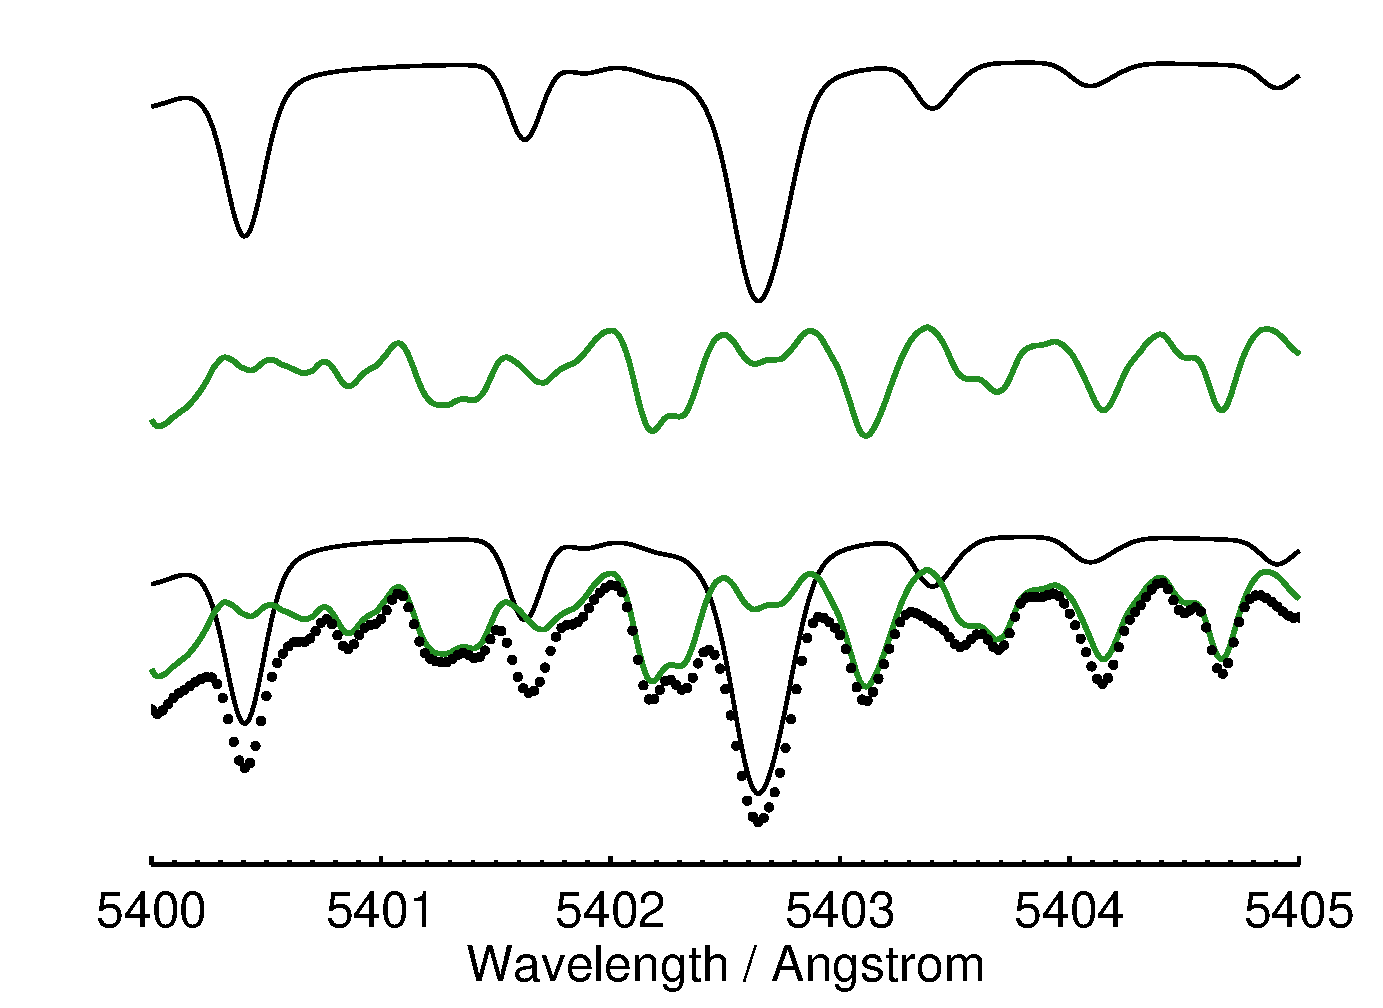
\includegraphics[scale=0.6]{doppler/forward_modeling.eps}
\caption{An illustration for the forward modeling process for
  iodine-calibrated stellar spectrum. The top black line represents
  the stellar reference spectrum (DSST), and the middle green line
  represents the iodine reference spectrum. Both reference spectra are
  convolved with an IP only for illustration purposes in order to have
  a clear match with the observed spectrum, plotted in black dots on
  the bottom. In practice, the reference spectra are multiplied {\it
    first} and then convolved with IP. \label{doppler:fig:modeling}}
\end{figure}
%----------------------------------------------------------------



%-------------------------------------------------------------------------------
\subsection{The Reference Spectra}

Ideally, the reference spectra are the ``ground truth" spectra,
i.e. the intrinsic spectra of the sources (e.g., the iodine cell, or
the star) without Doppler shift or being broadened by the
spectrometer. In reality, there is no way of knowing such ``ground
truth", so the reference spectra are empirically derived from
observations.

% how iodine atlas is made
The iodine reference spectrum, often referred to as the iodine atlas,
originates from a Fourier Transform Spectrometer scan of the iodine
cell illuminated by a continuum source. It is often of very high
signal-to-noise ratio (SNR) with high resolution (normally $\sim
500,000$ or larger). Therefore, it is generally regarded as basically
the ``ground truth" for the cell, especially for the purpose of
forward modeling lower-resolution ($\sim 60,000$) spectra. However,
there can be problems with the iodine atlas, for various reason. See
Chapter~\ref{chap:het} Section~\ref{het:sec:fts} for more on this
topic. The current FTS iodine atlas being used for \keck\ RV work is
from a scan in 1993, using the Babar FTS at NSO/KPNO, and so is the
atlas for \het. See Section~\ref{het:sec:fts} for more on iodine
reference spectra.

% how DSST is made
The stellar reference spectrum for any star, or internally to CPS
referred to as the Deconvolved Stellar Spectral Template (DSST), is
empirically derived from observed spectra of the target star. For most
of the CPS targets (bright stars), a few (4-5) observations of the
star with a narrower slit ($R \geq 80,000$) are taken without the
iodine cell in the light path. Then they are stacked together to boost
the SNR ($>500$), and then deconvolved with proper IPs derived from
bracketing B star $+$ iodine observations. The wavelength solution for
the DSST also comes from the bracketing B star $+$ iodine
observations. See Section~\ref{keck:sec:dsst} for more information and
problems related to DSSTs. For faint stars where obtaining stellar
template is expensive or unfeasible, \cite{2006ApJ...647..600J}
developed a technique where they ``morph" a synthetic stellar spectrum
or an existing DSST of another star with similar stellar properties to
fit the stellar iodine observation, and then they use this new morphed
DSST for RV extraction.


%-------------------------------------------------------------------------------
\subsection{The Functional Forms of the Instrumental Profile}\label{doppler:sec:ip}

The IP $\curlyp(x)$ can take many functional forms, and for \keck, an IP of sum of
gaussians works exceptionally well ($\chi^2 \sim 1$ for pure iodine
absorption line fit). The mathematical form for it is:
\beq
\curlyp_{\rm gaus}(x) = \sum A_n \exp{\left[\left(
    \frac{x-\mu_n}{\sigma_n} \right)^2\right]}. 
\eeq
$A_n$ stands for the amplitude for each gaussian component. $A_n$'s
are floated parameters for the fitter to optimize while $\mu_n$ and
$\sigma_n$ (i.e., positions and widths of the gaussians) have
empirically-optimized fixed values, depending on the instrument
setting of \keck\ (e.g., slit width). For \keck\ precise-RV mode (B5
decker, $\sim$60,000 resolution, with iodine cell in light path), the
IP contains 12 free parameters, $A_1, A_2, ..., A_{12}$, while $A_0$
is fixed to 1 (the big central gaussian) and $\mu_n, n=0,...,12$ and
$\sigma_n, n=0,...,12$ also have fixed values.

Another frequently used IP is the Gauss-Hermite (GH)
function, which is composed of gaussians multiplied by Hermite
polynomials $H_n$:
\beq
\curlyp_{\rm GH}(x) = \sum A_n u_n(x) = \sum A_n 
\left( \frac{2}{\pi w^2} \right)^{1/4} \frac{1}{\sqrt{n!2^2}} H_n
\left( \frac{\sqrt{2}x}{w} \right) \exp{\left[
    -\left(\frac{x}{w}\right) ^2  \right]}.
\eeq
Mathematically, any sum of gaussians can be decomposed into orthogonal
GH terms\footnote{See
  http://math.stackexchange.com/questions/28719/how-to-decompose-displaced-hermite-gauss-function-into-higher-order-hgs
  for an illustration, retrieved on March 18 2016.}, and therefore, in
principle, the GH IP should present a generic and flexible option for
IP choices. However, in reality, the least-$\chi^2$ solver is
extremely sensitive to the choices of initial guesses, even for
orthogonal bases. As a result, GH IP normally does not outperform sum
of gaussians (e.g., see work by \citealt{2013AAS...22114908V}). The GH
IP is what we use for extracting RVs from \het\ data. See
Chapter~\ref{chap:het} Section~\ref{het:sec:ip} for more.




%%%%%%%%%%%%%%%%%%%%%%%%%%%%%%%%%%%%%%%%%%%%%%%%%%%%%%%%%%%%%%%%%%%%%%%%%%%%%%
% structure of the code
\section{Code Structure and Work Flow}

Stellar spectra range from 5000\AA\ to 6200\AA. Chopped into
chunks. All working wavelengths are converted into vacuum. 


% Vanking!
